\documentclass{article}

\usepackage{amsmath,amssymb,amsthm}
\usepackage{mysymbols}
\usepackage{algorithm}
\usepackage{algorithmic}
\renewcommand{\algorithmicrequire}{\textbf{Input:}}
\renewcommand{\algorithmicensure}{\textbf{Output:}}
\usepackage{color}
\usepackage{tikz}
\usetikzlibrary{matrix}

\newcommand{\todo}[1]{(\textcolor{red}{TODO: #1})}

\newtheorem{Def}{Definition}
\newtheorem{Theo}{Theorem}
\newtheorem{Prop}{Proposition}
\newtheorem{Lemma}{Lemma}
\newtheorem{Coro}{Corollary}

\DeclareMathOperator{\Ext}{E}
\DeclareMathOperator{\Inv}{I}


\title{Rains' algorithm}

\begin{document}
\maketitle

Let $p$ be a prime, $q=p^d$ for an integer $d\ge1$, and $\F_q$ the
field with $q$ elements.

Rains' algorithm computes an isomorphism, or more generally an
embedding, between two given extensions $k_1/\F_q$ and $k_2/\F_q$. It
is a two phase algorithm like any other algorithm we know of:
\begin{enumerate}
\item Find generators $\eta_1$ of $k_1$ and $\eta_2$ of $k_2$ such
that there exists an isomorphisms $\phi:\eta_1\mapsto\eta_2$;
\item Compute a description of $\phi$, e.g.\ its change of basis
matrix.
\end{enumerate}

A notable feature of Rains' algorithm is that the generators
$\eta_1,\eta_2$ are normal elements. This can be used to improve the
second phase of the algorithm.

\section{First phase}

Let $n=[k_1:\F_q]=[k_2:\F_q]$. Rains' algorithm chooses the generators
$\eta_1,\eta_2$ in such a way that their minimal polynomial is
uniquely defined. In the simplest case, this is the $m$-th cyclotomic
polynomial, for an appropriately chosen $m$ depending upon $n$ and
$q$.

Rains' algorithm is a refinement of an algorithm by
Pinch~\cite{todo}. Pinch's idea is very simple: choose an $m$ such
that $k_1\isom\F_q[\mu_m]$, where $\mu_m$ is the group of $m$-th roots
of unity. Then any isomorphism $k_1\to k_2$ takes $\mu_m\subset
k_1^\ast$ to $\mu_m\subset k_2^\ast$. Choose $\eta_1$ and $\eta_2$ in
their respective fields to be generators of $\mu_m$, then test if
$\eta_1\mapsto\eta_2$ defines an isomorphism.

An easy case for Pinch's algorithm is when $n=m-1$. Indeed in this
case all the generators of $\mu_m$ are conjugate over $\F_q$, and
their minimal polynomial is the $m$-th cyclotomic polynomial
$\Phi_m$. Then, taking any $m$-th root of unity for $\eta_1$ and
$\eta_2$ will yield an isomorphism.

Things get more complicated when $m$ is larger. In this case, indeed,
one must chose $\eta_1$ and $\eta_2$ so that they are roots of the
same factor of $\Phi_m$. Pinch suggests picking random generators of
$\mu_m$ until a successful pair is found. To test if a pair is good,
Pinch advances to the second phase, then tests if the mapping induced
on the \emph{default} generators of $k_1$ and $k_2$ is acceptable.

Rains' improvement replaces the $m$-th roots of unity with their
Gaussian periods, thus avoiding Pinch's trial-and-error method. To
understand Rains' method, it is best to consider the structure of the
$m$-th roots of unity over the rationals. It is well known that
$\Q[\mu_m]/\Q$ is an abelian extension, and its Galois group can be
identified with $(\Z/m\Z)^\ast$. More generally, if $K$ is a number
field, $K[\mu_m]/K$ is an abelian extension with Galois group included
in $(\Z/m\Z)^\ast$.

We recall some basic concepts from algebraic number theory. Let $L/K$
be a Galois extension, and let $\frak{p}$ be a prime ideal of
$K$. Then $\frak{p}$ factors in $L$ as a product
\begin{equation} \frak{p} = \prod_{i=1}^s \frak{P}_i^e,
\end{equation}
where $e$ is the \emph{ramification degree}, $s$ is the
\emph{splitting degree}, and $f=[L:K]/se$ is the \emph{inertia
  degree}. When $e=1$ we say that the extension is unramified.

Let $K$ be a number field and $\frak{p}$ a prime in $K$ above $p$ such
that $\mathcal{O}_K/\frak{p}=\F_q$. Suppose that $K[\mu_m]/K$ is
unramified at $\frak{p}$, or equivalently that $p$ does not divide
$m$. Let $\frak{P}$ be a prime of $K[\mu_m]$ above $\frak{p}$. Then we
have a diagram
\begin{equation}
  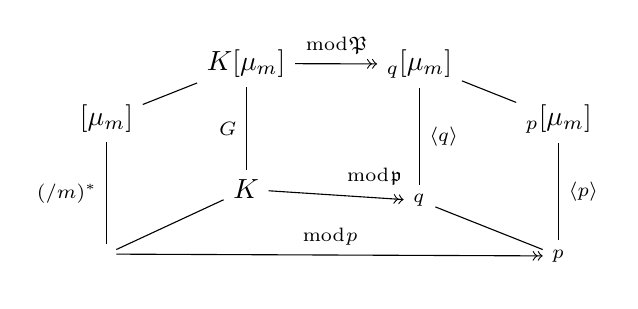
\begin{tikzpicture}[baseline=(current bounding box.base)]
    \node[matrix of math nodes, 
          column 1/.style={yshift=-2em}, 
          column 4/.style={yshift=-2em},
          column sep=2em,row sep=1em]{
      |(Ql)| \Q[\mu_m] & |(Kl)| K[\mu_m] &[1em] |(Fql)| \F_q[\mu_m] & |(Fpl)| \F_p[\mu_m]\\
      |(Q)| \Q & |(K)| K & |(Fq)| \F_q & |(Fp)| \F_p \\ };
    \begin{scope}[font=\scriptsize,auto]
      \draw (Q) edge node{$(\Z/m\Z)^\ast$} (Ql)
            (K) edge node{$G$} (Kl)
            (Fp) edge (Fq)
            (Fq) edge[right] node{$\langle q\rangle$} (Fql)
            (Fp) edge[right] node{$\langle p\rangle$} (Fpl)
            (Fpl) edge (Fql)
            (Q) edge (K)
            (Ql) edge (Kl);
      \draw[->>] (Kl) edge node{$\bmod\frak{P}$} (Fql)
                 (K) edge node{$\bmod\frak{p}$} (Fq)
                 (Q) edge node{$\bmod p$} (Fp);
    \end{scope}
  \end{tikzpicture}
\end{equation}
where we have identified the Galois groups with subgroups of
$(\Z/m\Z)^\ast$.

The Galois group $\langle q\rangle$ is the \emph{decomposition group}
of $\frak{P}/\frak{p}$. We have an inclusion $\langle q\rangle\subset
G\subset(\Z/m\Z)^\ast$ with orders
\begin{equation} \# G/\langle q\rangle = s,\qquad \#\langle q\rangle =
f = [K[\mu_m]:K]/s,
\end{equation}
where $s$ is the splitting degree and $f$ the inertia degree of
$\frak{p}$ in $K[\mu_m]$.

Pinch's algorithm performs better when $\langle q\rangle =
(\Z/m\Z)^\ast$. In this case, indeed, $\Phi_m$ is irreducible over
$\F_q$ and $\langle q\rangle$ acts transitively on the generators of
$\mu_m$. In Rains' algorithm the generators of $\mu_m$ are replaced by
their Gaussian periods, so that $\langle q\rangle$ acts transitively
on them.

\begin{Def}
  \label{def:period}
  Suppose that there is a subgroup $S\subset (\Z/m\Z)^\ast$ such that
  $(\Z/m\Z)^\ast = \langle q\rangle\times S$. For any generator
  $\zeta_m$ of $\mu_m$, define the Gaussian period
  \begin{equation}
    \label{eq:period} \eta_q(\zeta_m) = \sum_{\sigma\in
S}\zeta_m^\sigma.
\end{equation}
\end{Def}

In what follows we are going to write $\eta(\zeta_m)$ when the
subgroup $\langle q\rangle$ is clear from the context.

\begin{Prop}
  The Galois group $\Gal(\F_q[\mu_m]/\F_q)\isom\langle q\rangle$ acts
  transitively on the Gaussian periods $\eta(\zeta_m)$.
\end{Prop}
\begin{proof}
  Let $\tau\in\langle q\rangle$, then
  \begin{equation} \eta(\zeta_m)^\tau = \sum_{\sigma\in S}
\zeta_m^{\sigma\tau}.
  \end{equation}
  Since $(\Z/m\Z)^\ast=\langle q\rangle\times S$, any generator
  $\zeta_m'$ of $\mu_m$ can appear on the right hand side of the
  equation. Hence, $\langle q\rangle$ acts transitively on the set of
  all Gaussian periods.
\end{proof}

As a consequence, the minimal polynomial of $\eta(\zeta_m)$ is
uniquely defined and independent of $\zeta_m$.

\paragraph{Example.} Consider the extension $\F_8/\F_2$ of degree $3$,
which is generated by the $7$-th roots of unity. We have a decomposition $(\Z/7\Z)^\ast=\langle
2\rangle\times\langle-1\rangle$, and the cyclotomic
polynomial factors as 
\begin{equation}
  \Phi_7(x) = (x^3 + x + 1) (x^3 + x^2 + 1).
\end{equation}
For any root $\zeta_7$, we define the period
\begin{equation}
  \eta_2(\zeta_7) = \zeta_7+\zeta_7^{-1}.
\end{equation}
The three periods $\eta_2(\zeta_7)$, $\eta_2(\zeta_7)^2$ and
$\eta_2(\zeta_7)^4$ are all roots of the polynomial $x^3+x^2+1$ and
form a normal basis of $\F_8/\F_2$.

It remains to show that $\eta(\zeta_m)$ generates $\F_q[\mu_m]$,
however this is not true in general. Consider for example the case
where $\langle q\rangle$ is strictly contained in $\langle
p\rangle$. The period $\eta(\zeta_m)$ is stable under
$S\isom(\Z/m\Z)^\ast/\langle q\rangle$, hence it is also stable under
$\langle p\rangle/\langle q\rangle$, showing that $\eta(\zeta_m)$
belongs to a strict subfield of $\F_q[\mu_m]$. This is essentially the
only obstruction, as shows the following lemma.

\begin{Lemma}
  \label{th:generator} Let $m$ be an integer such that
  \begin{enumerate}
  \item $(\Z/m\Z)^\ast = \langle q\rangle \times S$ for some $S$,
  \item\label{th:generator:orthogonal} $\gcd(\euler(m), d)=1$,
  \item $m$ is squarefree \todo{I think this condition can be replaced
      by $\ord_\ell(q)\ne\ord_{\ell^2}(q)$ for any prime power
      $\ell^2$ dividing $m$}.
  \end{enumerate}

  The periods $\eta(\zeta_m)$ form a normal basis of $\F_q[\mu_m]$
  over $\F_q$.
\end{Lemma}
\begin{proof}
  Condition~\ref{th:generator:orthogonal} guarantees that $\langle
  p\rangle=\langle q\rangle$, hence $\eta(\zeta_m)$ generates
  $\F_q[\mu_m]/\F_q$ if and only if it generates
  $\F_p[\mu_m]/\F_p$. The rest of the proof is in Rains' paper.
\end{proof}

This corollary follows immediately.

\begin{Coro}
  \label{th:basic-rains}
  Let $k/\F_q$ be a degree $n$ extension. Let $m$ satisfy the
  conditions of Lemma~\ref{th:generator}, plus $\#\langle q\rangle =
  n$.  Then the periods $\eta(\zeta_m)$ form a normal basis of
  $k/\F_q$.
\end{Coro}

\paragraph{Remark.} The condition $(\Z/m\Z)^\ast = \langle
q\rangle\times S$ already implies that $\gcd(n,d)=1$. Indeed, by
hypothesis $p=sq^a\mod m$ for some $s\in S$ and $0\le a<n$, hence
$q=s^dq^{ad}\mod m$. But $q$ can be written in a unique way as a
product of an element of $S$ and an element of $\langle q\rangle$,
hence $s^d=1$ and $q^{ad-1}=1\mod m$. This implies that $n$ divides
$ad-1$, which in turn implies that $\gcd(n,d)=1$. In conclusion,
Rains' algorithm simply cannot handle the case where
$\gcd(n,d)=c\ne1$. A possible workaround is to compute a generator
$\eta(\zeta_m)$ of $k/\F_{p^{d/c}}$ instead: its minimal polynomial
will be uniquely defined over $\F_{p^{d/c}}$, but it will split into
$c$ factors over $\F_q$, thus requiring a trial-and error approach as
in Pinch's algorithm.

To summarize, the first phase of Rains' algorithm proceeds as follows.

\begin{enumerate}
\item Look for the smallest $m$ satisfying the conditions of
  Corollary~\ref{th:basic-rains};
\item Compute primitive $m$-th roots of unity $\zeta_1\in k_1$ and
  $\zeta_2\in k_2$;
\item Compute and return the Gaussian periods $\eta_i=\eta(\zeta_i)$.
\end{enumerate}

However the complexity of this algorithm is exponential in the worst
case, indeed the integer $m$ may be as large as $q^n-1$. There are two
possible ways to work around this limitation: work in a small field
extension of $k$, or replace $k^\ast$ with a different algebraic
group, e.g.\ an elliptic curve.

\section{Working in an extension field}

This is the original workaround suggested by Rains. The idea is to go
to a slightly larger field and use a trace to reduce to the desired
field. This widens the choices for $\ell$ enough to give a feasible
algorithm.

\begin{Coro}
  \label{th:rains}
  Let $k/\F_q$ be a degree $n$ extension. Let $m$ satisfy the
  conditions of Lemma~\ref{th:generator}, plus $\#\langle q\rangle =
  n\cdot o$.  Then the traces
  \begin{equation}
    \theta(\zeta_m) = \Tr_{\F_q[\mu_m]/k}\eta(\zeta_m) = \sum_{i=1}^o \eta_q(\zeta_m)^{q^{ni}}
  \end{equation}
  form a normal basis of $k/\F_q$.
\end{Coro}
\begin{proof}
  By Lemma~\ref{th:generator} the periods $\eta_q(\zeta_m)$ form a
  normal basis of $\F_q[\mu_m]$, which is a degree $o$ extension of
  $k$. By a classical result, the traces $\theta(\zeta_m)$ form a
  normal basis of $k$.
\end{proof}

The construction is summarized in the following diagram.
\begin{equation}
  \begin{tikzpicture}[baseline=(current bounding box.base)]
    \node[matrix of math nodes,
          every cell/.style={yshift=-2em*\pgfmatrixcurrentcolumn},
          column sep=2em]{
      |(Fqol)| \F_q[\eta(\zeta_m)] & |(Fql)| \F_q[\theta(\zeta_m)] & |(Fpl)| \F_p[\theta(\zeta_m)]\\
      |(Fqo)| \F_{q^o} & |(Fq)| \F_q & |(Fp)| \F_p \\ };
    \begin{scope}[font=\scriptsize,auto]
      \draw (Fp)  edge node{$d$} (Fq)
            (Fq)  edge node{$o$} (Fqo)
            (Fp)  edge node{$n$} (Fpl)
            (Fq)  edge node{$n$} (Fql)
            (Fqo) edge node{$n$} (Fqol)
            (Fpl) edge node{$d$} (Fql)
            (Fql) edge node{$o$} (Fqol);
    \end{scope}
  \end{tikzpicture}
\end{equation}

\paragraph{Example.} Let $p=24571$, and consider the extension
$\F_{p^3}/\F_p$. The $7$-th, $9$-th and $13$-th roots of unity are
already contained in $\F_p$. We find that $19$ is the smallest prime
power such that $p$ has order divisible by $3$, indeed $p=4\mod 19$
has order $9$ and $\Phi_{19}$ has $2$ factors of degree $9$. We have
a decomposition
$(\Z/19\Z)^\ast=\langle4\rangle\times\langle-1\rangle$, hence we
define the periods
\begin{equation}
  \eta_p(\zeta_{19}) = \zeta_{19} + \zeta_{19}^{-1}.
\end{equation}
These periods form a normal basis of $\F_{p^9}/\F_p$, and their
minimal polynomial is
\begin{equation}
  x^9 + x^8 - 8x^7 - 7x^6 + 21x^5 +
  15x^4 - 20x^3 - 10x^2 + 5x + 1.
\end{equation}
To obtain a normal basis of $\F_{p^3}/\F_p$ we compute the traces
\begin{equation}
  \theta(\zeta_{19}) = \eta_p(\zeta_{19}) + \eta_p(\zeta_{19})^{p^3} + \eta_p(\zeta_{19})^{p^6},
\end{equation}
we then verify that the minimal polynomial of the $\theta(\zeta_{19})$ is 
\begin{equation}
  x^3 + x^2 - 6x - 7.
\end{equation}
Observe that, by linearity, we have
\begin{equation}
  \def\z{\zeta_{19}}
  \theta(\zeta_{19}) = \z + \z^{-1} + \z^{4^3} + \z^{-4^3} + \z^{4^6} + \z^{-4^6},
\end{equation}
although this sum cannot be expressed as a Gaussian period.

Here we summarize the general algorithm.

\begin{enumerate}
\item Look for the smallest $m$ satisfying the conditions of
  Corollary~\ref{th:rains};
\item Construct extensions $K_1/k$ and $K_2/k$ of degree $o$;
\item Compute primitive $m$-th roots of unity $\zeta_1\in K_1$ and
  $\zeta_2\in K_2$;
\item Compute the Gaussian periods $\eta_i=\eta(\zeta_i)$;
\item Compute and return the traces $\theta_i=\theta(\zeta_i)$.
\end{enumerate}

\paragraph{Remark.} For efficiency, Rains requires $\gcd(n,o)=1$. In
this case, indeed, it is possible to construct the extension
$\F_q[\mu_m]/k$ using a polynomial with coefficients in $\F_p$ (recall
that $\gcd(d,o)=1$ is also necessary).

Observe that when $\gcd(n,o)=1$, from $(\Z/m\Z)^\ast=\langle
q\rangle\times S$ we deduce another decomposition
$(\Z/m\Z)^\ast=\langle q^o\rangle\times S'$ with $S\subset S'$. Then
defining the periods by means of $\langle q^o\rangle$ gives
$\eta_{q^o}(\zeta_m)=\theta(\zeta_m)$.


\section{Elliptic variant}

Replacing the multiplicative group $k^\ast$ with the group of points
of an elliptic curve was already suggested by Pinch. As for the
cyclotomic case, a trial-and-error approach is needed, unless one uses
carefully the decomposition of the Galois groups in play.

We look now for an elliptic curve $E/\F_q$ and an integer $m$ such
that the abscissas of the torsion group $E[m]$ generate an extension
of degree $n$ over $\F_q$.

Recall that for a given curve $E/\F_q$, its Frobenius endomorphism
$\pi$ is the map $(X:Y:Z)\mapsto(X^q:Y^q:Z^q)$. It satisfies a
quadratic equation $\pi^2-t\pi+q=0$, where the integer $t$ is called
the \emph{trace} of $\pi$ (or, by abuse of language, of $E$). The
number of rational points of $E/\F_q$ is equal to $q+1-t$. The minimal
equation of $\pi$ splits as $(\pi-\alpha)(\pi-\beta)$ in an imaginary
quadratic extension, and the number of rational points of $E/\F_{q^n}$
is equal to $q^n+1-(\alpha^n+\beta^n)$ for any integer $n$.

Most of the structure of $E$ is determined by the action of $\pi$,
which is in turn dictated by its minimal polynomial. For any integer
$m$ coprime with $p$, the group of $m$-torsion points $E[m]$ has rank
$2$, and for any fixed basis $\pi$ acts as a $2\times2$ matrix with
coefficients in $\Z/m\Z$.

\begin{Def}
  Let $E/\F_q$ be an elliptic curve and denote by $\pi$ its Frobenius
  endomorphism. A prime $\ell\ne2$ is called an \emph{Elkies prime}
  for $E$ if the minimal polynomial of $\pi$ splits over $\Z/\ell\Z$
  in two distinct factors.
\end{Def}

Equivalently, if $\ell$ is an Elkies prime, there is a basis of
$E[\ell]$ in which $\pi$ acts as a diagonal matrix
$\left(\begin{smallmatrix}\alpha&0\\0&\beta\end{smallmatrix}\right)$. For
any integer $n$, the Frobenius of $E/\F_{q^n}$ acts as the $n$-th
power of this matrix. Hence the extension of degree
$\min(\ord_\ell(\alpha),\ord_\ell(\beta))$ of $\F_q$ is the smallest
field containing a point of order $\ell$, and the extension of degree
$\ord_\ell(\pi)$ of $\F_q$ is the smallest extension containing all of
$E[\ell]$. By $\ell$-adic lifting, this is readily generalized to
powers of Elkies primes.

When trying to define elliptic periods, one must take into account a
phenomenon that does not happen with Gaussian periods. Elliptic curves
have non-trivial automorphisms which must be accounted for. We recall
the following classical theorem.

\begin{Prop}
  Let $E$ be an elliptic curve defined over a field $k$ of order $q$,
  and let $j$ be its $j$-invariant. The group of $k$-rational
  automorphisms of $E$, denoted $\Aut_k(E)$ has order
  \begin{itemize}
  \item $24$ if $j=0$ and $q=4\mod 6$,
  \item $12$ if $j=0$ and $q=9\mod 12$,
  \item $6$ if $j=0$ and $q=1 \mod 6$,
  \item $4$ if $j=1728$ and $q = 1,5 \mod 12$,
  \item $2$ in any other case.
  \end{itemize}
\end{Prop}

Now we can define the \emph{elliptic periods} in a similar way to the
Gaussian periods defined above.

\begin{Def}
  Let $E/\F_q$ be an elliptic curve, with $j\ne0$ in characteristic
  $2$ and $3$, and let $m$ be a power of an Elkies prime. Suppose that
  $\#\Aut_{\F_q}(E)$ divides $\euler(m)$, and identify $\Aut_{\F_q}(E)$ to a
  subgroup of $(\Z/m\Z)^\ast$. Let $\alpha\in(\Z/m\Z)^\ast$ be an
  eigenvalue of $\pi\bmod m$, and suppose that
  $(\Z/m\Z)^\ast/\Aut_{\F_q}(E)=\langle\alpha\rangle\times S$. For any
  primitive $m$-torsion point $P$ in the eigenspace of $\alpha$,
  define the elliptic period
  \begin{equation}
    \eta_\alpha(P) = \sum_{\sigma\in S} ([\sigma]P)_X^{\#\Aut_k(E)/2},
  \end{equation}
  where $[\sigma]P$ denotes scalar multiplication by $\sigma$, and
  $P_X$ denotes the abscissa of the point $P$.
\end{Def}

The case of $m$ a power of $p$ is also easy to deal with, as shown
below.

\begin{Def}
  Suppose $p\ne2$ \todo{is this really necessary?}, let $E/\F_q$ be an
  ordinary elliptic curve and let $k\ge1$. Let $t$ be the trace of
  $E$, and suppose that $(\Z/p^k\Z)^\ast/\Aut_{\F_q}(E)=\langle
  t\rangle\times S$. For any primitive $p^k$-torsion point $P\in E$,
  define the elliptic period
  \begin{equation}
    \eta_t(P) = \sum_{\sigma\in S} ([\sigma]P)_X.
  \end{equation}
\end{Def}

We deduce immediately the following proposition.

\begin{Prop}
  The Frobenius endomorphism $\pi$ acts transitively on the elliptic
  periods $\eta_\alpha(P)$ and $\eta_t(P)$.
\end{Prop}

Given $E$ and its trace, it is relatively easy to compute a basis for
$E[m]$, and then compute the eigenspaces of $\pi\bmod m$. However this
is a costly operation compared to other steps in Rains' algorithm,
thus we shall prefer to work with curves for which only one eigenspace
is defined over $\F_{q^n}$. Hence, we shall look for curves such
that $\ord_m(\beta)$ does not divide $\ord_m(\alpha)$.

Now we can formulate the main conjecture about elliptic periods.

\begin{Lemma}
  \label{th:elliptic-periods}
  Let $m$ be a prime power and let $t$ be an integer such that
  \begin{enumerate}
  \item $|t|<2\sqrt{q}$,
  \item $x^2-tx+q = (x-\alpha)(x-\beta) \mod m$,
  \item $(\Z/m\Z)^\ast = \langle\alpha\rangle \times S$,
  \item $\ord_m(\beta) \not| \ord_m(\alpha)$.
  \end{enumerate}
  Let $E/\F_q$ be an elliptic curve of trace $t$. Let $k$ be the
  smallest extension of $\F_q$ containing a point of order $m$. Then
  the periods $\eta_\alpha(P)$ for each $P\in E/k$ of order $m$ form a
  normal basis of $k$ over $\F_q$.
\end{Lemma}
\begin{proof}
  \todo{This is certainly false. It needs to be refined for non-prime,
    $m$, like the analogue for Gaussian periods.}
\end{proof}

\begin{Lemma}
  \label{th:elliptic-periods-p}
  Let $m$ be a power of $p$ and let $t$ be an integer such that
  \begin{enumerate}
  \item $|t|<2\sqrt{q}$,
  \item $(\Z/m\Z)^\ast = \langle t\rangle \times S$.
  \end{enumerate}
  Let $E/\F_q$ be an ordinary elliptic curve of trace $t$. Let $k$ be
  the smallest extension of $\F_q$ containing $E[m]$. Then the periods
  $\eta_t(P)$ for each $P\in E[m]$ form a normal basis of $k$ over
  $\F_q$.
\end{Lemma}
\begin{proof}
  \todo{}
\end{proof}

\begin{Coro}
  \label{th:elliptic-rains}
  Let $k/\F_q$ be a degree $n$ extension. Let $m$ satisfy the
  conditions of Lemma~\ref{th:elliptic-periods}
  (resp. Lemma~\ref{th:elliptic-periods-p}), plus $\#\langle
  \alpha\rangle = n$ (resp. $\#\langle t\rangle=n$).  Then the periods
  $\eta_\alpha(P)$ (resp. $\eta_t(P)$) form a normal basis of
  $k/\F_q$.
\end{Coro}

To summarize, here is the elliptic variant of Rains' algorithm.

\begin{enumerate}
\item Select the smallest odd prime power $m$ such that $n|\euler(m)$,
  $n\ne\euler(m)$ and $\gcd(\euler(m)/n,n)=1$;
\item Look for a curve $E/\F_q$ of trace $t$ such that $t\bmod m$
  satisfies the conditions of Corollary~\ref{th:elliptic-rains};
\item Compute primitive $m$-torsion points $P_1\in E/k_1$ and
  $P_2\in E/k_2$;
\item Compute and return the elliptic periods $\eta_i=\eta(P_i)$.
\end{enumerate}

\todo{It seems that the elliptic variant is not subject to the
  restriction $\euler(n,d)=1$. This needs to be checked.}

\todo{When $\F_q$ is too small, there are not enough curves to play
  with. We should start by taking a small extension.}

\paragraph{Example.}  Let $p=24571$ and consider the extension
$\F_{p^3}/\F_p$. We have seen before that the cyclotomic method
requires working in a degree $3$ extension. Using the elliptic method,
we can pick $m=31$, indeed $\ord_{31}(p)=15$, and we have a
decomposition
\begin{equation} 
  (\Z/31\Z)^\ast/\langle\pm1\rangle =
  \langle\alpha\rangle\times\langle16\rangle
\end{equation} 
for $\alpha=5,25$. To the two possible values for $\alpha$, are
associated two values for the trace $t=15,-4\mod m$. By counting the
points of the $2p+4$ curves defined over $\F_p$, we find that $3226$
of them (about $6.5\%$) have trace congruent to $15,-4$ modulo $31$,
which is consistent with the ratio $2/31$.

For example, Sage/Pari finds in about 10ms the curve
\begin{equation}
  E \;:\; y^2 = x^3 + 1274x - 5522
\end{equation}
of $j$-invariant $5$ and trace $232=15 \mod 31$. The curve has exactly
$31$ points of $31$-torsion in $\F_{p^3}$, and the periods
\begin{equation}
  \eta_\alpha(P_m) = \sum_{i=0}^{5-1}([16^i]P_m)_X
\end{equation}
form a normal basis of $\F_{p^3}/\F_p$, whose minimal polynomial is
\begin{equation}
  x^3 + 756x^2 + 687x + 8402.
\end{equation}


\section{Finding a suitable $m$}

\todo{Explain how to combine the factors of $n$ and mix algorithms
  using a linear integer program.}

\section{Powers of $2$}

\todo{The case $m=2^k$ is special for both algorithms. More
  investigation needed.}


\section{Bounds on $m$ and complexity analysis}

All variants are characterized by a \emph{search phase}, where we look
for the appropriate parameters $m$, $t$, etc., followed by a
\emph{computation phase}, where the periods are computed. In this
section we focus on the complexity of the computation phase. This is
usually the most expensive part of the algorithm, although the cost of
counting points of elliptic curves over $\F_q$ should not be neglected
for the elliptic variant.

We first need to give bounds for the integer $m$ computed in the
search phase. As discussed above, we can always reduce to the case
where $n$ and $m$ are prime powers. We can further restrict to the
case where $m$ is prime, as this dominates the asymptotic complexity.

As Rains points out, letting aside the constraints of
Lemmas~\ref{th:generator} and \ref{th:elliptic-periods}, for a given
$n$ we look for a prime $m$ of the form $an+1$. Heuristically one
expects to find such an $m$ in $O(n\log n)$, however the best bounds
(under GRH) are in $O(n^{2.4+\varepsilon})$. Taking into account the
additional constraints makes it very difficult to give even a
heuristic bound, however it seems reasonable to assume that $m$ will
still be in $O(n\log n)$ in practice \todo{try to give some
  arguments.}

Given the difficulty to formulate meaningful bounds on $m$, it is best
to give a detailed complexity analysis, depending upon $q,n$ and
$m$. Fortunately, these parameters can be efficiently computed before
running the full algorithm, thus a practical implementation can easily
choose among the different variants, or even change algorithm
altogether if no good parameters are found.

We express all complexities in number of operations in $\F_q$. We
write $\Ext(n)$ for the cost of multiplying two elements in $\F_{q^n}$
of degree at most $n$, and we assume that $\Ext$ is
superlinear. Usually it can be assumed that $\Ext(n)$ is in
$O(\Mult(n))$, where $\Mult(n)$ is the cost of multiplying two
polynomials of degree at most $n$ in $\F_q[X]$. Similarly we write
$\Inv(n)$ for the cost of inverting an element of $\F_{q^n}$; this is
usually assumed to be in $O(\Mult(n)\log n)$.

\subsection{Analysis of the basic cyclotomic algorithm}

The basic cyclotomic algorithm, where no finite field extension is
used, is very easy to analyze.

\begin{enumerate}
\item To compute an $m$-th root of unity, we repeat the following
  steps until one is found:
  \begin{itemize}
  \item We take a random element of $\F_{q^n}$ and we raise it to the
    $(q^n-1)/m$-th power;
  \item We raise the result to the powers $m/\ell$, for any prime
    $\ell$ dividing $m$, to test if it is a primitive root.
  \end{itemize}
  This is expected to succeed after $O(1)$ trials. Each trial requires
  $O(\Ext(n)n\log q)$ operations.
\item We then compute the period $\eta_q(\zeta_m)$, which involves
  $\euler(m)/n$ exponentiations with exponent at most $m$. Hence, the
  cost of this phase is $O((m\log m)\Ext(n)/n)$.
\end{enumerate}

Hence, the total cost is $O(\Ext(n)(n\log q + m\log m/n))$. As long as
$m\in o(n^2)$, the factors depending on $m$ are negligible, and we can
take $O(\Ext(n)n\log q)$ as complexity. This is at best quadratic in
$n$. Experimental evidence confirms the fact that the first step is
the most expensive part of the algorithm.


\subsection{Analysis of the cyclotomic algorithm with field
  extensions}

The algorithm using finite field extensions is only slightly more
complex than the previous one. Another parameter plays a role in the
complexity analysis: the degree $o$ of the auxiliary extension. This
degree is at most equal to $\euler(m)/n$.

\begin{enumerate}
\item We start by constructing the extension $\F_{q^{no}}$. If
  $\gcd(n,o)=1$, this can be done by means of a polynomial in
  $\F_p[X]$, and for small values of $o$ we can suppose that we have
  tabulated polynomials. For larger values of $o$, there are many
  different algorithms to choose among. Rather than entering into
  details, we assume that this step is in $O\left((no)^2\right)$,
  which is justifiable with the algorithms in~\cite{}.
\item We now compute an $m$-th root of unity in $\F_{q^{no}}$,
  proceeding as in the previous variant. The cost is $O(\Ext(no)no\log
  q)$.
\item Then we compute the period $\eta_{q^o}(\zeta_m)$. The cost is
  $O((m\log m)\Ext(no)/(no))$. 
\item Finally, we compute the trace $\theta(\zeta_m)$. By using the
  algorithm of~\cite{}, this can be done in
  $O\left((no)^2\right)$. The result is an element of $\F_{q^n}$, we
  suppose that changing representation to this field is in
  $O\left((no)^2\right)$, which is again justifiable by~\cite{}.
\end{enumerate}

Hence, the total cost is $O(\Ext(no)(no\log q + m\log m/(no)))$. As
long as $m\in o\left((no)^2\right)$, the worst case is $no=\euler(m)$,
which gives a cost of $O(\Ext(m)m\log q)$. This is at best quadratic
in $m$. Similarly the overhead of this algorithm compared to the basic
algorithm is at best quadratic in $o$. Experiments confirm this trend,
and show that the overhead becomes quickly prohibitive as $o$ grows.


\subsection{Analysis of the elliptic algorithm}

Finally we come to the elliptic variant. We shall see that its
complexity is closer to that of the basic cyclotomic algorithm, and
that in many circumstances this variant is preferable to the field
extension one.

We suppose that we already have computed an elliptic curve $E/\F_q$
with suitable parameters, and that we know its order over $\F_{q^n}$.

The algorithm needs to take random points on $E/\F_{q^n}$, however
this involves taking square roots in $\F_{q^n}$, which is
computationally expensive. Instead, we analyze a variant using only
$X$-coordinates, which is strictly equivalent for $n$ odd.

\begin{enumerate}
\item To compute a point of $m$-torsion, we repeat the following steps
  until one is found:
  \begin{itemize}
  \item We take a random element $x$ of $\F_{q^n}$ and we check that
    it is the abscissa of a point $P\in E$, otherwise we start over;
  \item Using Montgomery formulas~\cite{}, we compute the abscissa of
    $[\#E/m]P$;
  \item We multiply the result by $m/\ell$, for any prime $\ell$
    dividing $m$, to test if it is a primitive $m$-torsion point.
  \end{itemize}
  When $p\ne2$, testing if $x$ defines a point amounts to test if an
  element is a square in $\F_{q^n}$; this can be done in
  $O(n\Ext(n)\log q)$. When $p=2$, this amounts to compute a trace in
  $\F_{q^n}/\F_2$, which can be done in $O(n^2)$ by~\cite{}. Computing
  an addition or a duplication in $E$ using Montgomery formulas takes
  a constant number of multiplications and inversions in $\F_{q^n}$.
  Since $\#E\in O(q^n)$, the two other steps cost $O(n\Inv(n)\log
  q)$. We expect to find a point in $O(1)$ trials.
\item We then compute the period $\eta(P)$, which involves
  $\euler(m)/(2n)$ multiplication by a scalar smaller than
  $m/2$. Hence, the cost of this phase is $O((m\log m)\Inv(n)/n)$.  
\end{enumerate}

As before, if we suppose $m\in o(n^2)$, the total cost for the
algorithm is $O(n\Inv(n)\log q)$, which is at best quadratic. Although
the constant factors are larger than those implied in the cyclotomic
methods, there is a significant gain compared to the cyclotomic field
extension variant using a large degree $o$.

To summarize, as long as $m\ll n^2$, rather than stopping at the first
$m$ compatible with the field extension method, it may be worth to
look a little further for $m$'s compatible with the basic cyclotomic
method, or the elliptic method. A sensible balance between these
algorithms can only be established by practical experiments.


\end{document}




% Local Variables:
% ispell-local-dictionary:"american"
% End:

% LocalWords:  embeddings bilinear unramified endomorphism Elkies
